\documentclass[preprint, 12pt]{elsarticle}

% KU requirements
\usepackage[margin=2.5cm]{geometry}
\usepackage{setspace}
\onehalfspacing

% Temporary packages used while editing
\usepackage[usenames,dvipsnames]{color}

% Packages
\usepackage[colorlinks=true]{hyperref}
\usepackage{xspace}

% Options
\biboptions{authoryear}

% Custom commands
\newcommand{\Cree}{\emph{Cree}\xspace}

\begin{document}

\begin{frontmatter}

\title{\emph{Cree}: A modern toolbox for readymade economic experiments}
\author{Jonas K. Sekamane}
\journal{Supervised by Ulrik Haagen Nielsen.}
\address{{\color{red} First draft}}

\begin{abstract}
{\color{red} ...}
\end{abstract}
%\begin{keyword}Science \sep Publication \sep Complicated\end{keyword}

\end{frontmatter}


%% main text
\section{Introduction}
\label{S:Introduction}

This paper introduces a modern toolbox for readymade economic experiments called \Cree. \Cree takes advantage of the great advances in technology, in particular the new types of devices (smart-phones, tablets) and the availability of general-purpose software libraries. 

The great merit of \Cree is the very few restrictions it places on the equipment facing subjects. Few restrictions clear the way for much broader participation, strengthening the external validity of any experiment. \Cree experiments can be run in a myriad of settings, including laboratories, but also in \emph{extra-laboratory} settings such as classrooms, workplaces, or over the Internet \citep{Charness_Gneezy_Kuhn_2013}. With \Cree the computer-equipped laboratory is no longer a necessity -- lowering the overall costs of conducting economic experiments. The researcher can still choose to provide subjects with devices, but can just as easily let subjects use their own devices. 

\Cree is build using web technologies. Content is structured using the markup language \emph{HTML}. The layout and presentation across different screen sizes is archived with the style sheet language \emph{CSS}. And all logic is constructed using the programming language \emph{JavaScript}. All web browsers interpret these three cornerstone languages and render pages accordingly. Subjects participate in \Cree experiments though a web browser. Because \Cree is fundamentally native to the web browser, it avoids many of the restrictions, that other toolboxes suffer from.

In addition there is a vibrant ecosystem surrounding these web technologies. \Cree exploits this ecosystem and takes full advantage of the software libraries that exist. This provides stability, flexibility, and makes it easy to set up and run economic experiments. Fore instances, \Cree uses the software library \emph{Node.js} to run the server and handle networking issues. The asynchronous architecture of \emph{Node.js} gives \Cree the flexibility to handle real-time events, which many other toolboxes is not capable of. With this flexibility \Cree can run everything, from simple dictator game experiments, to highly sophisticated auction experiments. \Cree is a framework that provides the tools to handle many of the otherwise mundane, complicated or manually tasks required to set up and run economic experiments.

Technological advances opens up a new path, however the path is not without obstacles. This paper explores and discusses how to handle these obstacles. Some obstacles are alleviated through appropriate technical design of the toolbox. Other obstacles require actions taken by the researcher.

{\color{red}... Explain why you repeatedly refer to studies on Mechanical Turk ...}

\section{Requirements}
\label{S:Requirements}

\subsection{System requirements}

\Cree requires a server, ie. any computer with \emph{Node.js} installed\footnotemark[1]. \Cree has several dependencies -- because it is built on general-purpose software libraries -- however all of these dependencies are automatically installed, or come pre-bundled, with \Cree. The server will need to be connected to the devices used by the subject, either through the internet or though a local network (eg. WiFi). 

\begin{figure}[h!]
  \caption{Schematic overview of the network setup with server and clients}
  \centering
    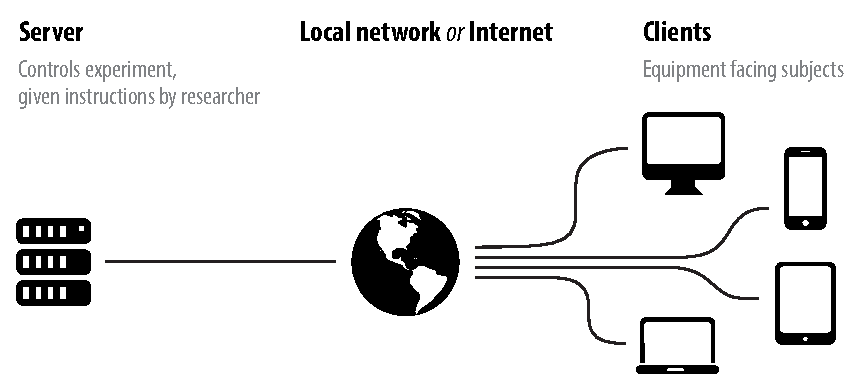
\includegraphics[width=\textwidth]{figures/setup}
\end{figure}

Subjects access \Cree experiments though an web browser. Any modern web browser will suffice\footnotemark[2], which means that subjects can participate in experiments using smart-phones, tablets, or any computer (Windows, Mac, Linux). Every subject will need a device. The researcher can choose to provide devices, or have subjects use their own personal devices.

\footnotetext[1]{Node.js is easily installed from \url{http://nodejs.org}.}

\footnotetext[2]{A modern web browser is either: IE version 9+, Chrome current version, Firefox current version, OSX Safari version 5.1+, Opera version 12.1+, iOS Safari version 6.1+, or Android Browser version 4.0+. The browser must allow JavaScript, which all browsers due by default. \Cree automatically check that these requirements are met, before the subject is allowed to enter the experiment.}

\subsection{Alternative toolboxes}

\emph{z-Tree} is currently the commonly used toolbox for conducting economic experiments. The development of \emph{z-Tree} started in 1995 and has been updated continuously \citep{Fischbacher_2007}. However the foundation and guiding principles of \emph{z-Tree} is based on the technology that was available two decades ago. Several other toolboxes exist that can run economic experiments. Below I divide the the toolboxes into four categories based on the restrictions they places on the equipment facing subjects:

\begin{table}[h!]
\begin{tabular}{ l p{0.7\textwidth} }
{\bf Application:} & z-Tree, E-Prime, ESI/ICES Software \\
{\bf Requires Python:} & UAA-PEET \\
{\bf Requires Java:} & BoXS, EconPort, Multistage, Comlab, Aton, JessX, JAuctions, JMarkets, SWIEE \\
{\bf Browser native:} & SoPHIE, Willow, jsPsych, Tatool, QRTEngine, WebExp, WEXTOR, VeconLab \\
\end{tabular}
\end{table}

Toolboxes, such as \emph{z-Tree}, are applications. They are written for a specific operating system, and will only run on that specific operating system. All toolboxes in this category requires Microsoft Windows. These applications are not easily ported to other computer operating systems. And they will require a complete restructuring -- focused on optimising screen sizes and battery life -- if they are every to run on smart-phones or tablets. In addition, applications will have to be downloaded (and installed) on the computer facing subjects, before they can participate in experiments. This requirement hinders subjects from using their personal devices.

The second category contains toolboxes written in \emph{Python}. Python is platform independent, so these toolboxes can run on several operating systems, but they require that Python is installed on the equipment facing subjects\footnotemark[3]. These toolboxes also require downloading software.

\footnotetext[3]{Python can be packaged into stand-alone applications. These stand-alone applications can run on equipment where Python is not installed.}

Toolboxes in the third category are written in \emph{Java}. These are less restrictive, since subjects can participate in experiments though a web browser that has the Java-plugin. Thus there is no need to predownload or preinstall software on the equipment facing subjects. While the Java-plugin is widely distributed, it is not universal\footnotemark[4]. And increasing concerns regarding security issues with the Java-plugin has lead browsers manufactures to implement various warnings and hindrances\footnotemark[5]. 

\footnotetext[4]{A Millward Brown survey from 2011 found a penetration rate of 73\% on PCs in mature markets. Source: \url{http://www.adobe.com/mena_en/products/flashplatformruntimes/statistics.html}. This is also mimicked on the server-side with only 0.1\% of websites using Java. Source: \url{http://w3techs.com/technologies/overview/client_side_language/all}. The Java-plugin is not supported on iOS nor Android. Source: \url{http://www.java.com/en/download/faq/java_mobile.xml}.}
 
\footnotetext[5]{Eg. due to security concerns by default the Java-plugin is disabled in Google Chrome version 42 (released April 2015). Source: \url{https://www.java.com/en/download/faq/chrome.xml}.}

The fourth category of toolboxes run natively in the web browser, without the need for any browser plug-ins or predownloaded software. These toolboxes place the same low restrictions on the equipment facing subjects as \Cree. However, none of these toolboxes currently support simultaneous real-time interaction between subjects -- ie. it is impossible to design experiments where subjects continuously provide input, while continuously and simultaneously receives feedback from the other subjects. Some toolboxes support sequential decision making, while others completely lack interaction among subjects.

\section{Running experiments}
\label{S:Running}

\section{Expected results}
\label{S:Results}

\section{Designing experiments}
\label{S:Designing}

\section{Conclusion}
\label{S:Conclusion}


%% References
\bibliographystyle{apalike}
\raggedright
\singlespacing
\bibliography{references.bib}

\end{document}